\documentclass[conference]{IEEEtran}
\usepackage{amsmath,amssymb,amsthm}
\usepackage{booktabs}
\usepackage{graphicx}
\usepackage{algorithm}
\usepackage{algpseudocode}
\usepackage{xspace}
\usepackage{url}
\usepackage{cite}
\newcommand{\KReal}{398}
\newcommand{\EpReal}{8}
\newcommand{\certfracRealmcar}{23.8}
\newcommand{\imputeerrRealmcar}{7.2}
\newcommand{\imputeerronunkRealmcar}{9.4}
\newcommand{\imputeerroncertRealmcar}{0.0}
\newcommand{\certwrongRealmcar}{0}
\newcommand{\violRealmcar}{110}
\newcommand{\ndecReal}{1672}
\newcommand{\nitemsReal}{15920}
\newcommand{\aucRealmcarrandom}{0.099}
\newcommand{\cnRealmcarrandom}{0.951}
\newcommand{\daucRealmcarrandom}{0.596}
\newcommand{\ciRealmcarrandom}{[0.585, 0.605]}
\newcommand{\winsRealmcarrandom}{8/8}
\newcommand{\aucRealmcarwidest}{0.484}
\newcommand{\cnRealmcarwidest}{0.462}
\newcommand{\daucRealmcarwidest}{0.211}
\newcommand{\ciRealmcarwidest}{[0.204, 0.218]}
\newcommand{\winsRealmcarwidest}{8/8}
\newcommand{\aucRealmcardegree}{0.485}
\newcommand{\cnRealmcardegree}{0.627}
\newcommand{\daucRealmcardegree}{0.210}
\newcommand{\ciRealmcardegree}{[0.204, 0.216]}
\newcommand{\winsRealmcardegree}{8/8}
\newcommand{\aucRealmcarlocal}{0.462}
\newcommand{\cnRealmcarlocal}{0.504}
\newcommand{\daucRealmcarlocal}{0.234}
\newcommand{\ciRealmcarlocal}{[0.224, 0.242]}
\newcommand{\winsRealmcarlocal}{8/8}
\newcommand{\aucRealmcarvoiOne}{0.620}
\newcommand{\cnRealmcarvoiOne}{0.386}
\newcommand{\daucRealmcarvoiOne}{0.076}
\newcommand{\ciRealmcarvoiOne}{[0.071, 0.080]}
\newcommand{\winsRealmcarvoiOne}{8/8}
\newcommand{\aucRealmcarseaq}{0.695}
\newcommand{\cnRealmcarseaq}{0.352}
\newcommand{\aucRealmcarseaqmyopic}{0.643}
\newcommand{\cnRealmcarseaqmyopic}{0.372}
\newcommand{\daucRealmcarseaqmyopic}{0.052}
\newcommand{\ciRealmcarseaqmyopic}{[0.048, 0.056]}
\newcommand{\winsRealmcarseaqmyopic}{8/8}
\newcommand{\aucRealmcarseaqmax}{0.689}
\newcommand{\cnRealmcarseaqmax}{0.359}
\newcommand{\daucRealmcarseaqmax}{0.006}
\newcommand{\ciRealmcarseaqmax}{[0.004, 0.007]}
\newcommand{\winsRealmcarseaqmax}{8/8}
\newcommand{\certfracReallate}{22.1}
\newcommand{\imputeerrReallate}{8.2}
\newcommand{\imputeerronunkReallate}{10.5}
\newcommand{\imputeerroncertReallate}{0.0}
\newcommand{\certwrongReallate}{0}
\newcommand{\violReallate}{62}
\newcommand{\aucReallaterandom}{0.086}
\newcommand{\cnReallaterandom}{0.933}
\newcommand{\daucReallaterandom}{0.651}
\newcommand{\ciReallaterandom}{[0.646, 0.656]}
\newcommand{\winsReallaterandom}{8/8}
\newcommand{\aucReallatewidest}{0.659}
\newcommand{\cnReallatewidest}{0.313}
\newcommand{\daucReallatewidest}{0.077}
\newcommand{\ciReallatewidest}{[0.073, 0.081]}
\newcommand{\winsReallatewidest}{8/8}
\newcommand{\aucReallatedegree}{0.553}
\newcommand{\cnReallatedegree}{0.439}
\newcommand{\daucReallatedegree}{0.183}
\newcommand{\ciReallatedegree}{[0.175, 0.191]}
\newcommand{\winsReallatedegree}{8/8}
\newcommand{\aucReallatelocal}{0.512}
\newcommand{\cnReallatelocal}{0.434}
\newcommand{\daucReallatelocal}{0.224}
\newcommand{\ciReallatelocal}{[0.217, 0.231]}
\newcommand{\winsReallatelocal}{8/8}
\newcommand{\aucReallatevoiOne}{0.694}
\newcommand{\cnReallatevoiOne}{0.273}
\newcommand{\daucReallatevoiOne}{0.042}
\newcommand{\ciReallatevoiOne}{[0.039, 0.045]}
\newcommand{\winsReallatevoiOne}{8/8}
\newcommand{\aucReallateseaq}{0.736}
\newcommand{\cnReallateseaq}{0.257}
\newcommand{\aucReallateseaqmyopic}{0.706}
\newcommand{\cnReallateseaqmyopic}{0.266}
\newcommand{\daucReallateseaqmyopic}{0.030}
\newcommand{\ciReallateseaqmyopic}{[0.028, 0.033]}
\newcommand{\winsReallateseaqmyopic}{8/8}
\newcommand{\aucReallateseaqmax}{0.717}
\newcommand{\cnReallateseaqmax}{0.274}
\newcommand{\daucReallateseaqmax}{0.019}
\newcommand{\ciReallateseaqmax}{[0.018, 0.020]}
\newcommand{\winsReallateseaqmax}{8/8}
\newcommand{\certfracRealmnar}{20.3}
\newcommand{\imputeerrRealmnar}{13.7}
\newcommand{\imputeerronunkRealmnar}{17.2}
\newcommand{\imputeerroncertRealmnar}{0.0}
\newcommand{\certwrongRealmnar}{0}
\newcommand{\violRealmnar}{228}
\newcommand{\aucRealmnarrandom}{0.142}
\newcommand{\cnRealmnarrandom}{0.937}
\newcommand{\daucRealmnarrandom}{0.612}
\newcommand{\ciRealmnarrandom}{[0.602, 0.623]}
\newcommand{\winsRealmnarrandom}{8/8}
\newcommand{\aucRealmnarwidest}{0.578}
\newcommand{\cnRealmnarwidest}{0.398}
\newcommand{\daucRealmnarwidest}{0.175}
\newcommand{\ciRealmnarwidest}{[0.167, 0.183]}
\newcommand{\winsRealmnarwidest}{8/8}
\newcommand{\aucRealmnardegree}{0.499}
\newcommand{\cnRealmnardegree}{0.597}
\newcommand{\daucRealmnardegree}{0.254}
\newcommand{\ciRealmnardegree}{[0.245, 0.264]}
\newcommand{\winsRealmnardegree}{8/8}
\newcommand{\aucRealmnarlocal}{0.493}
\newcommand{\cnRealmnarlocal}{0.464}
\newcommand{\daucRealmnarlocal}{0.260}
\newcommand{\ciRealmnarlocal}{[0.251, 0.269]}
\newcommand{\winsRealmnarlocal}{8/8}
\newcommand{\aucRealmnarvoiOne}{0.702}
\newcommand{\cnRealmnarvoiOne}{0.314}
\newcommand{\daucRealmnarvoiOne}{0.051}
\newcommand{\ciRealmnarvoiOne}{[0.049, 0.054]}
\newcommand{\winsRealmnarvoiOne}{8/8}
\newcommand{\aucRealmnarseaq}{0.753}
\newcommand{\cnRealmnarseaq}{0.283}
\newcommand{\aucRealmnarseaqmyopic}{0.721}
\newcommand{\cnRealmnarseaqmyopic}{0.308}
\newcommand{\daucRealmnarseaqmyopic}{0.032}
\newcommand{\ciRealmnarseaqmyopic}{[0.029, 0.035]}
\newcommand{\winsRealmnarseaqmyopic}{8/8}
\newcommand{\aucRealmnarseaqmax}{0.744}
\newcommand{\cnRealmnarseaqmax}{0.293}
\newcommand{\daucRealmnarseaqmax}{0.009}
\newcommand{\ciRealmnarseaqmax}{[0.007, 0.010]}
\newcommand{\winsRealmnarseaqmax}{8/8}
\newcommand{\KSynth}{400}
\newcommand{\EpSynth}{12}
\newcommand{\certfracSynthmcar}{23.7}
\newcommand{\imputeerrSynthmcar}{8.8}
\newcommand{\imputeerronunkSynthmcar}{11.5}
\newcommand{\imputeerroncertSynthmcar}{0.0}
\newcommand{\certwrongSynthmcar}{0}
\newcommand{\violSynthmcar}{27}
\newcommand{\ndecSynth}{1680}
\newcommand{\nitemsSynth}{16000}
\newcommand{\aucSynthmcarrandom}{0.109}
\newcommand{\cnSynthmcarrandom}{0.947}
\newcommand{\daucSynthmcarrandom}{0.570}
\newcommand{\ciSynthmcarrandom}{[0.565, 0.575]}
\newcommand{\winsSynthmcarrandom}{12/12}
\newcommand{\aucSynthmcarwidest}{0.466}
\newcommand{\cnSynthmcarwidest}{0.485}
\newcommand{\daucSynthmcarwidest}{0.213}
\newcommand{\ciSynthmcarwidest}{[0.209, 0.217]}
\newcommand{\winsSynthmcarwidest}{12/12}
\newcommand{\aucSynthmcardegree}{0.478}
\newcommand{\cnSynthmcardegree}{0.669}
\newcommand{\daucSynthmcardegree}{0.201}
\newcommand{\ciSynthmcardegree}{[0.197, 0.205]}
\newcommand{\winsSynthmcardegree}{12/12}
\newcommand{\aucSynthmcarlocal}{0.453}
\newcommand{\cnSynthmcarlocal}{0.541}
\newcommand{\daucSynthmcarlocal}{0.226}
\newcommand{\ciSynthmcarlocal}{[0.223, 0.230]}
\newcommand{\winsSynthmcarlocal}{12/12}
\newcommand{\aucSynthmcarvoiOne}{0.615}
\newcommand{\cnSynthmcarvoiOne}{0.422}
\newcommand{\daucSynthmcarvoiOne}{0.064}
\newcommand{\ciSynthmcarvoiOne}{[0.062, 0.066]}
\newcommand{\winsSynthmcarvoiOne}{12/12}
\newcommand{\aucSynthmcarseaq}{0.679}
\newcommand{\cnSynthmcarseaq}{0.379}
\newcommand{\aucSynthmcarseaqmyopic}{0.638}
\newcommand{\cnSynthmcarseaqmyopic}{0.405}
\newcommand{\daucSynthmcarseaqmyopic}{0.041}
\newcommand{\ciSynthmcarseaqmyopic}{[0.039, 0.043]}
\newcommand{\winsSynthmcarseaqmyopic}{12/12}
\newcommand{\aucSynthmcarseaqmax}{0.669}
\newcommand{\cnSynthmcarseaqmax}{0.389}
\newcommand{\daucSynthmcarseaqmax}{0.010}
\newcommand{\ciSynthmcarseaqmax}{[0.009, 0.011]}
\newcommand{\winsSynthmcarseaqmax}{12/12}
\newcommand{\certfracSynthlate}{22.4}
\newcommand{\imputeerrSynthlate}{10.3}
\newcommand{\imputeerronunkSynthlate}{13.2}
\newcommand{\imputeerroncertSynthlate}{0.0}
\newcommand{\certwrongSynthlate}{0}
\newcommand{\violSynthlate}{18}
\newcommand{\aucSynthlaterandom}{0.091}
\newcommand{\cnSynthlaterandom}{0.922}
\newcommand{\daucSynthlaterandom}{0.636}
\newcommand{\ciSynthlaterandom}{[0.630, 0.642]}
\newcommand{\winsSynthlaterandom}{12/12}
\newcommand{\aucSynthlatewidest}{0.651}
\newcommand{\cnSynthlatewidest}{0.317}
\newcommand{\daucSynthlatewidest}{0.075}
\newcommand{\ciSynthlatewidest}{[0.073, 0.077]}
\newcommand{\winsSynthlatewidest}{12/12}
\newcommand{\aucSynthlatedegree}{0.545}
\newcommand{\cnSynthlatedegree}{0.462}
\newcommand{\daucSynthlatedegree}{0.182}
\newcommand{\ciSynthlatedegree}{[0.178, 0.186]}
\newcommand{\winsSynthlatedegree}{12/12}
\newcommand{\aucSynthlatelocal}{0.522}
\newcommand{\cnSynthlatelocal}{0.437}
\newcommand{\daucSynthlatelocal}{0.205}
\newcommand{\ciSynthlatelocal}{[0.201, 0.209]}
\newcommand{\winsSynthlatelocal}{12/12}
\newcommand{\aucSynthlatevoiOne}{0.685}
\newcommand{\cnSynthlatevoiOne}{0.285}
\newcommand{\daucSynthlatevoiOne}{0.042}
\newcommand{\ciSynthlatevoiOne}{[0.041, 0.043]}
\newcommand{\winsSynthlatevoiOne}{12/12}
\newcommand{\aucSynthlateseaq}{0.727}
\newcommand{\cnSynthlateseaq}{0.269}
\newcommand{\aucSynthlateseaqmyopic}{0.697}
\newcommand{\cnSynthlateseaqmyopic}{0.279}
\newcommand{\daucSynthlateseaqmyopic}{0.030}
\newcommand{\ciSynthlateseaqmyopic}{[0.029, 0.031]}
\newcommand{\winsSynthlateseaqmyopic}{12/12}
\newcommand{\aucSynthlateseaqmax}{0.706}
\newcommand{\cnSynthlateseaqmax}{0.287}
\newcommand{\daucSynthlateseaqmax}{0.021}
\newcommand{\ciSynthlateseaqmax}{[0.019, 0.023]}
\newcommand{\winsSynthlateseaqmax}{12/12}
\newcommand{\certfracSynthmnar}{14.4}
\newcommand{\imputeerrSynthmnar}{19.8}
\newcommand{\imputeerronunkSynthmnar}{23.1}
\newcommand{\imputeerroncertSynthmnar}{0.0}
\newcommand{\certwrongSynthmnar}{0}
\newcommand{\violSynthmnar}{72}
\newcommand{\aucSynthmnarrandom}{0.143}
\newcommand{\cnSynthmnarrandom}{0.938}
\newcommand{\daucSynthmnarrandom}{0.554}
\newcommand{\ciSynthmnarrandom}{[0.548, 0.561]}
\newcommand{\winsSynthmnarrandom}{12/12}
\newcommand{\aucSynthmnarwidest}{0.510}
\newcommand{\cnSynthmnarwidest}{0.460}
\newcommand{\daucSynthmnarwidest}{0.188}
\newcommand{\ciSynthmnarwidest}{[0.185, 0.191]}
\newcommand{\winsSynthmnarwidest}{12/12}
\newcommand{\aucSynthmnardegree}{0.475}
\newcommand{\cnSynthmnardegree}{0.676}
\newcommand{\daucSynthmnardegree}{0.222}
\newcommand{\ciSynthmnardegree}{[0.219, 0.225]}
\newcommand{\winsSynthmnardegree}{12/12}
\newcommand{\aucSynthmnarlocal}{0.464}
\newcommand{\cnSynthmnarlocal}{0.530}
\newcommand{\daucSynthmnarlocal}{0.233}
\newcommand{\ciSynthmnarlocal}{[0.228, 0.238]}
\newcommand{\winsSynthmnarlocal}{12/12}
\newcommand{\aucSynthmnarvoiOne}{0.647}
\newcommand{\cnSynthmnarvoiOne}{0.394}
\newcommand{\daucSynthmnarvoiOne}{0.051}
\newcommand{\ciSynthmnarvoiOne}{[0.049, 0.052]}
\newcommand{\winsSynthmnarvoiOne}{12/12}
\newcommand{\aucSynthmnarseaq}{0.698}
\newcommand{\cnSynthmnarseaq}{0.356}
\newcommand{\aucSynthmnarseaqmyopic}{0.666}
\newcommand{\cnSynthmnarseaqmyopic}{0.384}
\newcommand{\daucSynthmnarseaqmyopic}{0.031}
\newcommand{\ciSynthmnarseaqmyopic}{[0.030, 0.032]}
\newcommand{\winsSynthmnarseaqmyopic}{12/12}
\newcommand{\aucSynthmnarseaqmax}{0.686}
\newcommand{\cnSynthmnarseaqmax}{0.369}
\newcommand{\daucSynthmnarseaqmax}{0.012}
\newcommand{\ciSynthmnarseaqmax}{[0.011, 0.013]}
\newcommand{\winsSynthmnarseaqmax}{12/12}
\newcommand{\KRealHet}{398}
\newcommand{\EpRealHet}{12}
\newcommand{\certfracRealHetmcar}{26.2}
\newcommand{\imputeerrRealHetmcar}{7.1}
\newcommand{\imputeerronunkRealHetmcar}{9.7}
\newcommand{\imputeerroncertRealHetmcar}{0.0}
\newcommand{\certwrongRealHetmcar}{0}
\newcommand{\violRealHetmcar}{191}
\newcommand{\ndecRealHet}{1672}
\newcommand{\nitemsRealHet}{15920}
\newcommand{\aucRealHetmcarrandom}{0.105}
\newcommand{\cnRealHetmcarrandom}{0.944}
\newcommand{\daucRealHetmcarrandom}{0.570}
\newcommand{\ciRealHetmcarrandom}{[0.562, 0.578]}
\newcommand{\winsRealHetmcarrandom}{12/12}
\newcommand{\aucRealHetmcarwidest}{0.409}
\newcommand{\cnRealHetmcarwidest}{0.511}
\newcommand{\daucRealHetmcarwidest}{0.266}
\newcommand{\ciRealHetmcarwidest}{[0.263, 0.269]}
\newcommand{\winsRealHetmcarwidest}{12/12}
\newcommand{\aucRealHetmcardegree}{0.255}
\newcommand{\cnRealHetmcardegree}{0.755}
\newcommand{\daucRealHetmcardegree}{0.421}
\newcommand{\ciRealHetmcardegree}{[0.414, 0.425]}
\newcommand{\winsRealHetmcardegree}{12/12}
\newcommand{\aucRealHetmcarlocal}{0.412}
\newcommand{\cnRealHetmcarlocal}{0.552}
\newcommand{\daucRealHetmcarlocal}{0.263}
\newcommand{\ciRealHetmcarlocal}{[0.255, 0.271]}
\newcommand{\winsRealHetmcarlocal}{12/12}
\newcommand{\aucRealHetmcarvoiOne}{0.582}
\newcommand{\cnRealHetmcarvoiOne}{0.450}
\newcommand{\daucRealHetmcarvoiOne}{0.093}
\newcommand{\ciRealHetmcarvoiOne}{[0.089, 0.098]}
\newcommand{\winsRealHetmcarvoiOne}{12/12}
\newcommand{\aucRealHetmcarseaq}{0.675}
\newcommand{\cnRealHetmcarseaq}{0.376}
\newcommand{\aucRealHetmcarseaqmyopic}{0.611}
\newcommand{\cnRealHetmcarseaqmyopic}{0.432}
\newcommand{\daucRealHetmcarseaqmyopic}{0.064}
\newcommand{\ciRealHetmcarseaqmyopic}{[0.061, 0.068]}
\newcommand{\winsRealHetmcarseaqmyopic}{12/12}
\newcommand{\aucRealHetmcarseaqmax}{0.662}
\newcommand{\cnRealHetmcarseaqmax}{0.392}
\newcommand{\daucRealHetmcarseaqmax}{0.013}
\newcommand{\ciRealHetmcarseaqmax}{[0.011, 0.014]}
\newcommand{\winsRealHetmcarseaqmax}{12/12}
\newcommand{\certfracRealHetlate}{24.3}
\newcommand{\imputeerrRealHetlate}{8.5}
\newcommand{\imputeerronunkRealHetlate}{11.4}
\newcommand{\imputeerroncertRealHetlate}{0.0}
\newcommand{\certwrongRealHetlate}{0}
\newcommand{\violRealHetlate}{122}
\newcommand{\aucRealHetlaterandom}{0.094}
\newcommand{\cnRealHetlaterandom}{0.925}
\newcommand{\daucRealHetlaterandom}{0.619}
\newcommand{\ciRealHetlaterandom}{[0.613, 0.625]}
\newcommand{\winsRealHetlaterandom}{12/12}
\newcommand{\aucRealHetlatewidest}{0.606}
\newcommand{\cnRealHetlatewidest}{0.343}
\newcommand{\daucRealHetlatewidest}{0.108}
\newcommand{\ciRealHetlatewidest}{[0.104, 0.112]}
\newcommand{\winsRealHetlatewidest}{12/12}
\newcommand{\aucRealHetlatedegree}{0.296}
\newcommand{\cnRealHetlatedegree}{0.567}
\newcommand{\daucRealHetlatedegree}{0.417}
\newcommand{\ciRealHetlatedegree}{[0.400, 0.433]}
\newcommand{\winsRealHetlatedegree}{12/12}
\newcommand{\aucRealHetlatelocal}{0.483}
\newcommand{\cnRealHetlatelocal}{0.462}
\newcommand{\daucRealHetlatelocal}{0.231}
\newcommand{\ciRealHetlatelocal}{[0.224, 0.237]}
\newcommand{\winsRealHetlatelocal}{12/12}
\newcommand{\aucRealHetlatevoiOne}{0.648}
\newcommand{\cnRealHetlatevoiOne}{0.308}
\newcommand{\daucRealHetlatevoiOne}{0.066}
\newcommand{\ciRealHetlatevoiOne}{[0.062, 0.070]}
\newcommand{\winsRealHetlatevoiOne}{12/12}
\newcommand{\aucRealHetlateseaq}{0.714}
\newcommand{\cnRealHetlateseaq}{0.281}
\newcommand{\aucRealHetlateseaqmyopic}{0.668}
\newcommand{\cnRealHetlateseaqmyopic}{0.298}
\newcommand{\daucRealHetlateseaqmyopic}{0.045}
\newcommand{\ciRealHetlateseaqmyopic}{[0.043, 0.048]}
\newcommand{\winsRealHetlateseaqmyopic}{12/12}
\newcommand{\aucRealHetlateseaqmax}{0.691}
\newcommand{\cnRealHetlateseaqmax}{0.300}
\newcommand{\daucRealHetlateseaqmax}{0.023}
\newcommand{\ciRealHetlateseaqmax}{[0.021, 0.025]}
\newcommand{\winsRealHetlateseaqmax}{12/12}
\newcommand{\certfracRealHetmnar}{21.4}
\newcommand{\imputeerrRealHetmnar}{14.3}
\newcommand{\imputeerronunkRealHetmnar}{18.2}
\newcommand{\imputeerroncertRealHetmnar}{0.0}
\newcommand{\certwrongRealHetmnar}{0}
\newcommand{\violRealHetmnar}{415}
\newcommand{\aucRealHetmnarrandom}{0.152}
\newcommand{\cnRealHetmnarrandom}{0.930}
\newcommand{\daucRealHetmnarrandom}{0.567}
\newcommand{\ciRealHetmnarrandom}{[0.556, 0.577]}
\newcommand{\winsRealHetmnarrandom}{12/12}
\newcommand{\aucRealHetmnarwidest}{0.482}
\newcommand{\cnRealHetmnarwidest}{0.462}
\newcommand{\daucRealHetmnarwidest}{0.237}
\newcommand{\ciRealHetmnarwidest}{[0.227, 0.248]}
\newcommand{\winsRealHetmnarwidest}{12/12}
\newcommand{\aucRealHetmnardegree}{0.257}
\newcommand{\cnRealHetmnardegree}{0.745}
\newcommand{\daucRealHetmnardegree}{0.462}
\newcommand{\ciRealHetmnardegree}{[0.452, 0.470]}
\newcommand{\winsRealHetmnardegree}{12/12}
\newcommand{\aucRealHetmnarlocal}{0.440}
\newcommand{\cnRealHetmnarlocal}{0.518}
\newcommand{\daucRealHetmnarlocal}{0.279}
\newcommand{\ciRealHetmnarlocal}{[0.269, 0.288]}
\newcommand{\winsRealHetmnarlocal}{12/12}
\newcommand{\aucRealHetmnarvoiOne}{0.648}
\newcommand{\cnRealHetmnarvoiOne}{0.389}
\newcommand{\daucRealHetmnarvoiOne}{0.071}
\newcommand{\ciRealHetmnarvoiOne}{[0.069, 0.073]}
\newcommand{\winsRealHetmnarvoiOne}{12/12}
\newcommand{\aucRealHetmnarseaq}{0.719}
\newcommand{\cnRealHetmnarseaq}{0.323}
\newcommand{\aucRealHetmnarseaqmyopic}{0.673}
\newcommand{\cnRealHetmnarseaqmyopic}{0.374}
\newcommand{\daucRealHetmnarseaqmyopic}{0.046}
\newcommand{\ciRealHetmnarseaqmyopic}{[0.044, 0.048]}
\newcommand{\winsRealHetmnarseaqmyopic}{12/12}
\newcommand{\aucRealHetmnarseaqmax}{0.708}
\newcommand{\cnRealHetmnarseaqmax}{0.334}
\newcommand{\daucRealHetmnarseaqmax}{0.011}
\newcommand{\ciRealHetmnarseaqmax}{[0.010, 0.013]}
\newcommand{\winsRealHetmnarseaqmax}{12/12}
\newcommand{\stK}{398}
\newcommand{\stT}{580}
\newcommand{\stEvents}{476,479}
\newcommand{\stRestated}{721}
\newcommand{\stViol}{1364}
\newcommand{\tputpoint}{135.5}
\newcommand{\tputcert}{71.3}
\newcommand{\tputrecomp}{2.9}
\newcommand{\stcertTotal}{749,892}
\newcommand{\stcertEmitted}{100.0}
\newcommand{\stcertWrong}{397}
\newcommand{\stcertWrongPct}{0.05}
\newcommand{\stcertDelay}{0.84}
\newcommand{\stcertOnTime}{62.9}
\newcommand{\stcertRev}{415}
\newcommand{\stcertFlag}{415}
\newcommand{\stpointTotal}{749,892}
\newcommand{\stpointEmitted}{100.0}
\newcommand{\stpointWrong}{18,001}
\newcommand{\stpointWrongPct}{2.40}
\newcommand{\stpointDelay}{0.00}
\newcommand{\stpointOnTime}{100.0}
\newcommand{\stpointRev}{19,851}
\newcommand{\stpointFlag}{0}
\newcommand{\stwaitTotal}{749,892}
\newcommand{\stwaitEmitted}{100.0}
\newcommand{\stwaitWrong}{344}
\newcommand{\stwaitWrongPct}{0.05}
\newcommand{\stwaitDelay}{3.50}
\newcommand{\stwaitOnTime}{3.0}
\newcommand{\stwaitRev}{344}
\newcommand{\stwaitFlag}{344}

\newtheorem{definition}{Definition}
\newtheorem{lemma}{Lemma}
\newtheorem{theorem}{Theorem}
\newtheorem{proposition}{Proposition}
\newcommand{\seaq}{SEAQ\xspace}
\newcommand{\T}{\textsf{T}\xspace}
\newcommand{\F}{\textsf{F}\xspace}
\newcommand{\U}{\textsf{U}\xspace}

\begin{document}
\title{Certified Threshold Alerts over Incomplete Multi-Source Streams:\\ Sound Abstention and Shared-Evidence Acquisition}

\author{\IEEEauthorblockN{Adishree Gupta}
\IEEEauthorblockA{Dept. of CSE, PES University\\Bengaluru, India\\ORCID: 0009-0002-5909-135X}
\and
\IEEEauthorblockN{Akshat}
\IEEEauthorblockA{Dept. of CSE, PES University\\Bengaluru, India\\ORCID: 0009-0008-2977-6298}
\and
\IEEEauthorblockN{Shylaja S S}
\IEEEauthorblockA{Dept. of CSE, PES University\\Bengaluru, India\\ORCID: 0000-0003-2628-8973}}

\maketitle

\begin{abstract}
Monitoring systems evaluate threshold predicates over windowed aggregates (``alert if the 5-day traded volume of a
stock exceeds 1.5$\times$ its norm''). Their inputs come from several sources and are routinely late, missing, or
reported only approximately. Conventional engines fill the gaps with point estimates and emit alerts that may be
wrong and are later silently reversed. We study the threshold-decision workload under interval-annotated evidence and make
three contributions. (i)~\emph{Semantics and operator:} a three-valued certified alert (true / false / insufficient).
Its certified outcomes hold in every completion consistent with the evidence, \emph{provided the declared bounds
contain the true values}. It is maintained incrementally
over sliding windows and roll-ups in $O(\deg(i))$ per evidence change, with explicit detection of contradictory
evidence. (ii)~\emph{Theory of acquisition:} under adversarial evidence, no proper subset of a decision's uncertain
inputs can guarantee its resolution, so worst-case budgeted acquisition over shared evidence contains Densest-$k$-Subgraph
and is NP-hard. For window-structured workloads, however, we give an exact
strongly polynomial planner that maximises the number of alerts guaranteed to be settled. With industry roll-ups, an
exact ILP shows that the planner's plan stays within 1\% of the optimum. On the real panel it settles up to
$1.9\times$ more than the best heuristic plan at low budgets, in about one second. (iii)~\emph{\seaq}, an adaptive acquisition policy that scores each uncertain input by the share of
uncertainty it removes, summed over all undetermined decisions it feeds. A controlled fan-out benchmark shows that its
gains come from width normalisation rather than from sharing, and that they vanish at high fan-out. On a real panel of \KReal{} Indian
equities reported independently by two exchanges (NSE and BSE), and on a synthetic workload, \seaq{} gives the largest area
under the resolution-vs-budget curve in all nine settings (real, synthetic and heterogeneous-cost workloads, each under three missingness models). Its paired gain over the
best baseline (myopic value of information) is 0.042--0.076 AUC on real data, and over a TRAPP-style widest-first policy it is
0.077--0.211. In a 460-day stream replay, certified alerts were wrong at emission
\stcertWrongPct\% of the time versus \stpointWrongPct\% for imputation. We show that every such error requires a
restatement or a violated declared bound. Certified alerts are emitted \stcertDelay{} days after window close on average, against
\stwaitDelay{} days for waiting for complete data. We also report where the approach does not help.
\end{abstract}

\section{Introduction}
\label{sec:intro}
\textbf{Motivating example.} Market-surveillance pipelines, such as the capstone system that motivated this work
(an NSE equity-surveillance pipeline built by one of the authors), raise volume alerts of the form
\[
\textstyle Q_{k}^{W,c}:\quad \sum_{t'=t-W+1}^{t}\big(v^{\text{NSE}}_{k,t'}+v^{\text{BSE}}_{k,t'}\big) > c\cdot W\cdot \mathrm{med}_k
\]
for each stock $k$, plus the same predicate rolled up to industries. The inputs arrive from two exchanges,
often late; some come from secondary channels (vendor feeds, OCR of broadcast tickers) only as approximate
readings. At window close a conventional engine replaces a missing input by an estimate (a median or last value) and
emits a Boolean. In our replay that alert was wrong \stpointWrong{} times out of \stpointTotal{} emitted decisions
(Section~\ref{sec:stream}), and \stpointRev{} emitted decisions were later reversed with no indication of why.

The underlying database problem is broader than finance. It arises when (a)~queries are \emph{decisions}
(HAVING/threshold predicates, alerts, SLA checks) rather than numbers; (b)~evidence for an input is partial but
\emph{bounded}; and (c)~inputs are \emph{shared} by many decisions through overlapping windows, several thresholds and
roll-ups. Two questions follow: \emph{which decisions are already settled by the evidence?} and, for the rest,
\emph{which missing inputs should be fetched first when fetching costs money or time?}

\textbf{What is known.} Bounding query answers over incomplete data is well studied: certain answers and
three-valued logic~\cite{imielinski1984,libkin2016}, UA-DBs and AU-DBs that propagate attribute-level
bounds~\cite{feng2019uadb,feng2021audb}, and probabilistic databases~\cite{dalvi2004,antova2007}. Choosing which
values to refresh so that an aggregate meets a precision target was solved for a \emph{single} query by
TRAPP~\cite{olston2000trapp}. Probing for imprecise data~\cite{cheng2003} and oracle-based query-oriented
cleaning~\cite{bergman2015qoco} also address single queries or SPJ answers. None of these treats the
\emph{multi-decision} acquisition problem in which one input feeds many threshold decisions with different slacks.
In that setting the per-query optimum is not the global optimum.

\textbf{Core insight.} The certified state of a SUM-threshold decision is determined only by two counters
$(L_d,U_d)$, so it can be maintained exactly and cheaply. Acquisition, however, has a sharp negative structure:
under worst-case evidence a decision is guaranteed to be resolved only when \emph{all} its uncertain inputs are known
(Lemma~\ref{lem:nopartial}). Myopic ``resolve-in-one-probe'' scores are therefore mostly zero and mislead, which we
also measure (Table~\ref{tab:acq}). A score that credits each input with the \emph{fraction} of every undetermined
decision's residual width it removes does better. It is simple and can be maintained over the sparse decision--input
incidence.

\textbf{Contributions} (each checked in Section~\ref{sec:eval}):
\begin{enumerate}
\item A three-valued certified threshold operator over interval-annotated windowed aggregates with roll-ups. It
has a soundness guarantee, narrowing-monotonicity, contradiction detection, and $O(\deg(i))$ incremental
maintenance (Section~\ref{sec:model}).
\item Lemma~\ref{lem:nopartial} (no partial worst-case certificate), Theorem~\ref{thm:hard} (worst-case budgeted
acquisition with arbitrary sharing is NP-hard, also adaptively), and Theorem~\ref{thm:dp}: a strongly polynomial exact optimiser for guaranteed-resolution planning on window workloads, and an exact ILP
reference for roll-ups. On the real panel it settles up to $1.9\times$ more
alerts than the best heuristic plan at low budgets (Sections~\ref{sec:theory},~\ref{sec:wc}).
\item \seaq, a shared-evidence acquisition policy, with ablations and a controlled fan-out benchmark that isolate
where its gains come from, and where they disappear (Sections~\ref{sec:seaq},~\ref{sec:fanout}).
\item CQP, a DuckDB-backed prototype that keeps all state in SQL and implements the operator, retractions, \seaq{}
and the exact planner. It passes 16 correctness, equivalence and numerical-soundness tests, runs a deterministic end-to-end demo, and is
benchmarked against full SQL recomputation on the real panel (Section~\ref{sec:cqp}).
\item An evaluation on a real two-exchange panel and a synthetic workload under MCAR, late-arrival and adversarial
(MNAR) missingness. It covers an end-to-end stream replay with restatements, and throughput against conventional
and recompute engines (Section~\ref{sec:eval}). Code and the frozen development log are released with the
submission (Section~\ref{sec:repro}).
\end{enumerate}

\section{Model and Certified Semantics}
\label{sec:model}
\begin{definition}[Evidence]
An \emph{item} $i$ has an unknown true value $v_i\in\mathbb{R}_{\ge 0}$ and evidence $[\ell_i,h_i]$. An item
is \emph{exact} if $\ell_i=h_i$, \emph{approximate} if it carries a reading with a declared relative error
$\epsilon$, and \emph{missing} if it carries only a declared domain bound $[0,B_i]$. The \emph{soundness assumption}
is $v_i\in[\ell_i,h_i]$. The width is $w_i=h_i-\ell_i$.
\end{definition}
Any modality whose extractor reports a bounded error (OCR digits with a checksum, a derived value with a
tolerance, a vendor feed with a known deviation bound) reduces to this form. Unbounded corruption does not, and it is
handled by contradiction detection below.

\begin{definition}[Threshold decision]
A decision $d$ is a pair $(S_d,\theta_d)$ asking whether $\sum_{i\in S_d}v_i>\theta_d$. Let
$L_d=\sum_{S_d}\ell_i$, $U_d=\sum_{S_d}h_i$, $W_d=U_d-L_d$. Its certified state is $\T$ if $L_d>\theta_d$,
$\F$ if $U_d\le\theta_d$, and $\U$ (insufficient) otherwise.
\end{definition}
A workload is a sparse incidence matrix $M\in\{0,1\}^{|D|\times|I|}$. Sliding windows of length $W$ place an item in
$W$ consecutive decisions per threshold level, and roll-ups (industry sums) add further rows. COUNT reduces to
SUM over indicator items. MIN/MAX use the analogous bounds $\max_i \ell_i$ and $\max_i h_i$, maintained with
monotone deques; we evaluate SUM only.

\begin{proposition}[Soundness and monotonicity]
\label{prop:sound}
(a)~If every item satisfies the soundness assumption, a decision in state $\T$ ($\F$) is true (false) for the true
values, and indeed for every completion consistent with the evidence. (b)~Replacing $[\ell_i,h_i]$ by a sub-interval
never changes a certified state. (c)~If new evidence $[\ell'_i,h'_i]$ is disjoint from $[\ell_i,h_i]$, the old or
the new evidence violates the soundness assumption.
\end{proposition}
\begin{proof}
(a)~$L_d\le\sum v_i\le U_d$. (b)~Narrowing increases $L_d$ and decreases $U_d$, so $L_d>\theta$ and $U_d\le\theta$
are preserved. (c)~A single $v_i$ cannot lie in two disjoint intervals.
\end{proof}
Part (a) says certification is the \emph{certain-answer} semantics~\cite{imielinski1984,libkin2016} specialised to
aggregate thresholds; it is also what an AU-DB-style bound propagation would give~\cite{feng2021audb}. We claim no novelty for
(a)--(c). They fix the contract on which the operator and the acquisition problem rest. The \emph{operator}
reacts to a contradiction (case (c)) by flagging the item and \emph{retracting} every emitted decision whose
certification no longer holds, instead of silently flipping it.

\textbf{Incremental maintenance.} When item $i$ changes from $[\ell,h]$ to $[\ell',h']$, the operator adds
$\ell'-\ell$ to $L_d$ and $h'-h$ to $U_d$ for every $d$ with $M_{di}=1$. With a column-indexed incidence (or, for
sliding windows, an implicit index range) this costs $O(\deg(i))$ time. The state test is $O(1)$ per touched
decision. Storage is two counters per decision and two bounds per item, i.e.\ about twice a point engine. A
recompute engine that re-sums each touched decision costs $O(\sum_{d\ni i}|S_d|)$ instead.

\section{Theory of Acquisition}
\label{sec:theory}
A \emph{probe} of item $i$ costs $c_i>0$ and reveals $v_i$. Given budget $B$, which items should be probed?
\begin{lemma}[No partial worst-case certificate]
\label{lem:nopartial}
Let $d$ satisfy $L_d\le\theta_d<U_d$ (i.e.\ state $\U$) and let $P$ be a proper subset of its non-exact items. Then there are values
$v_i\in[\ell_i,h_i]$ for $i\in P$ after which $d$ is still in state $\U$.
\end{lemma}
\begin{proof}
Let $A=\sum_{i\in P}w_i<W_d$. Revealing values for $P$ shifts $L_d$ up by some $s\in[0,A]$ and $U_d$ down by $A-s$,
and every $s\in[0,A]$ is attainable by choosing the $v_i$. The new state is $\U$ iff
$L_d+s\le\theta_d<U_d-A+s$, i.e.\ $s\in(\theta_d-U_d+A,\;\theta_d-L_d]$. This interval has length $W_d-A>0$. Its
upper end $\theta_d-L_d\ge0$, and its lower end $\theta_d-U_d+A<A$. Hence it meets $[0,A]$; $s=0$ works when
$\theta_d=L_d$ because then $\theta_d-U_d+A<0$.
\end{proof}
So no non-adaptive plan short of probing \emph{every} uncertain input of $d$ can guarantee resolving $d$, however
wide the probed items are. Guarantees are thus purely combinatorial. Exact items ($w_i=0$) are irrelevant to
the statement. A randomized search over 200{,}000 small instances (including zero-width items and ties
$\theta_d=L_d$) found no counterexample to the constructive witness (\texttt{verify\_theory.py}).
\begin{theorem}[Hardness]
\label{thm:hard}
Given decisions over shared items, unit costs and an integer $k$, choosing $k$ items to maximise the number of
decisions guaranteed (for all consistent values) to be resolved is NP-hard.
\end{theorem}
\begin{proof}
Reduce from Densest-$k$-Subgraph~\cite{feige2001dks}. Given $G=(V,E)$, create one item per vertex with evidence
$[0,1]$ and one decision per edge $\{u,v\}$ with $S_d=\{u,v\}$ and $\theta_d=1$, so $L_d=0<1<2=U_d$. By
Lemma~\ref{lem:nopartial}, $d$ is guaranteed resolved iff both endpoints are probed, and probing both resolves
it. Hence the number of guaranteed-resolved decisions equals the number of edges induced by the chosen $k$
vertices.
\end{proof}
\emph{Adaptivity does not help in the reduction}: an adversary that answers $0.5$ to every probe leaves each edge
with an unprobed endpoint in state $\U$ ($L=0.5\le1<1.5=U$). So the adaptive worst-case version is NP-hard on the
same family; we verified the correspondence exhaustively on random 6-vertex graphs. The reduction uses arbitrary
pairwise sharing. Pure sliding windows over one series have interval structure and are not covered by it. The next
result shows that this structure makes the problem tractable.

\textbf{Guaranteed-resolution planning (GR).} Given budget $B$, choose probes so as to maximise the number of
undetermined decisions that are resolved \emph{for every consistent outcome}. The result is a plan whose payoff can be
committed to before any data arrive: ``with budget $B$ we will settle at least $N^*(B)$ alerts''. By
Lemma~\ref{lem:nopartial}, a decision is guaranteed iff all its uncertain items are probed. Partially probing a time
slot of a series (one key-day with several sources) never helps, so slots are atomic with cost $c_t\ge0$.
\begin{theorem}[Exact GR for window workloads]
\label{thm:dp}
Suppose every decision on key $k$ covers a contiguous range of time slots of $k$ (sliding windows of any lengths and
any number of thresholds), and keys share no items. Then GR is solvable exactly in
$O\big(\sum_k m_k^2\,|D_k| + |D|^2\big)$ arithmetic operations (additions and comparisons on costs), where $m_k$ is the
number of uncertain slots of key $k$ and $D_k$ its undetermined decisions. The bound holds for arbitrary nonnegative
real (or binary-encoded rational) costs and budgets, so the algorithm is strongly polynomial.
\end{theorem}
\begin{proof}
Fix key $k$ with uncertain slots $u_1<\dots<u_m$ and sentinels $u_0,u_{m+1}$. Each undetermined decision maps to an
index range $[p_d,q_d]$ of uncertain slots. It is guaranteed iff no \emph{unprobed} uncertain slot lies in
$[p_d,q_d]$, i.e.\ iff the range lies strictly between two consecutive unprobed indices. Any plan is therefore
described by its increasing sequence of unprobed indices $0=i_0<i_1<\dots<i_r=m+1$. Its cost is
$\sum_{\ell}\mathrm{cost}(i_{\ell-1},i_\ell)$ with $\mathrm{cost}(i,j)=\sum_{i<l<j}c_l$, and its value is
$\sum_\ell G(i_{\ell-1},i_\ell)$ with $G(i,j)=|\{d: i<p_d,\ q_d<j\}|$. Each guaranteed decision is counted exactly once,
in the unique gap that contains its range. Both cost and value decompose over consecutive pairs. We index the table by \emph{value}, which is an integer
bounded by $|D_k|$, rather than by budget:
$\mathrm{mc}[j][v]=\min_{i<j}\mathrm{mc}[i][v-G(i,j)]+\mathrm{cost}(i,j)$ is the minimum cost of a plan whose last
unprobed index is $j$ and that guarantees $v$ decisions. This takes $O(m^2|D_k|)$ operations, with $G$ tabulated in
$O(m^2)$ from 2-D prefix counts. Keys are independent, so the global minimum cost $g(v)$ of guaranteeing $v$ decisions is
the min-plus convolution of the per-key tables. This costs $O(|D|^2)$ overall, and the answer is $\max\{v: g(v)\le B\}$.
No step depends on the magnitude of costs or of $B$.
\emph{Slot atomicity is without loss of optimality.} An uncertain item of slot $t$ matters only to decisions
containing $t$, and each such decision needs \emph{all} uncertain items of $t$. Dropping the probed items of an
incompletely probed slot therefore keeps the value and does not increase the cost. Item-level costs thus aggregate into
$c_t=\sum$ of the slot's uncertain item costs, and zero-cost items are harmless. \emph{Bit complexity:} every number
the algorithm stores is a sum of at most $m_k$ (or $\sum_k m_k$) input costs, so its encoding length exceeds that of
the inputs by $O(\log\sum_k m_k)$ bits. Space is $O(m_k|D_k|)$ per key plus $O(|D|)$ for the convolution.
\end{proof}
\emph{Complexity by cost model.} The budget-indexed variant of the same recurrence (our first implementation) is
pseudo-polynomial, $O(\sum_k m_k^2B)$. It is polynomial for unit or polynomially bounded integer costs (then
$B\le\sum c$), but not in the binary encoding of $B$. The value-indexed form removes this dependence. It also returns
the whole cost-versus-guarantee frontier $g(\cdot)$ in one pass, which is what a budget planner needs.
We distinguish three workload classes. In \emph{Class A} (independent keys, any overlapping windows and
thresholds), GR is strongly polynomial (Thm.~\ref{thm:dp}). \emph{Class B} (industry or laminar roll-ups over Class A)
has open complexity; we solve it exactly by ILP and observe near-optimality of the Class-A plan only on the tested
instances. In \emph{Class C} (arbitrary sharing), GR is NP-hard (Thm.~\ref{thm:hard}). Theorems~\ref{thm:hard}
and~\ref{thm:dp} together draw the tractability line \emph{inside} the monitoring workload.
Overlapping windows of mixed lengths, repeated thresholds, and several sources per slot are strongly polynomial.
Arbitrary sharing is NP-hard. Industry roll-ups lie in between: their decisions span the slots of many keys over a time
interval (a laminar key family times intervals), which breaks the per-key decomposition. We do \emph{not} settle their
complexity. Instead we solve them exactly with a 0-1 ILP whose group-day variables $z_{g,t}\le x_{k,t}$ keep the model
linear in the size of the incidence (Section~\ref{sec:wc}). We checked both implementations against exhaustive search. The budget-indexed one (\texttt{wcdp.py}) matched on 3{,}000
random integer-cost instances. The value-indexed one (\texttt{wcdp\_sp.py}) matched on 2{,}000 real-cost instances, on
the integer cases, and on 300 two-key combinations, and the ILP matched on 200 arbitrary-sharing instances. A further audit used \emph{exact rational
arithmetic} and brute force over \emph{individual source items}, which also tests slot atomicity. It covered 1{,}500
instances, including zero-cost items, zero budgets, empty decision sets, and identical and nested ranges
(\texttt{verify\_exact.py}). There were no mismatches. Random testing is evidence, not proof; the proof above is the
argument. The dynamic program itself uses a standard
gap-decomposition technique. What we contribute is the GR formulation for certified decisions and the tractability
boundary it reveals.
Densest-$k$-Subgraph is also hard to approximate under standard complexity assumptions (see~\cite{feige2001dks} and
follow-up work). We therefore do not pursue worst-case guarantees. Instead we optimise the \emph{empirical} resolution
curve with an adaptive policy and measure it. Adaptive acquisition for a single linear threshold function is a
stochastic Boolean function evaluation problem~\cite{deshpande2014sbfe}. The multi-decision, shared-input version
studied here is what our policy targets.

\section{\seaq: Shared-Evidence Acquisition}
\label{sec:seaq}
For an undetermined decision $d$ define the gaps $g^L_d=\theta_d-L_d$ and $g^U_d=U_d-\theta_d$, with
$W_d=g^L_d+g^U_d$. Two natural per-input signals exist:
\begin{itemize}
\item \emph{One-probe resolution probability.} If $v_i\sim\mathrm{Unif}[\ell_i,h_i]$, probing $i$ resolves $d$
with probability exactly
$P_1(d,i)=\big(\max(0,w_i-g^L_d)+\max(0,w_i-g^U_d)\big)/w_i$, since $d$ becomes $\T$ iff $v_i-\ell_i>g^L_d$ and $\F$
iff $h_i-v_i\ge g^U_d$. This is the myopic value-of-information (VOI) score.
\item \emph{Progress share.} $w_i/W_d$, the fraction of $d$'s residual uncertainty that probing $i$ removes. By
Lemma~\ref{lem:nopartial}, resolution needs the residual width to collapse below the gap, so progress counts even
when $P_1=0$.
\end{itemize}
\seaq{} probes, in batches of $b$, the items with the largest
\begin{equation}
\mathrm{score}(i)=\frac{1}{c_i}\sum_{d:\,M_{di}=1,\ \mathrm{state}(d)=\U}\frac{w_i}{W_d}.
\label{eq:seaq}
\end{equation}
After each batch the revealed values update $(L_d,U_d)$ incrementally and resolved decisions drop out of the sum.
The sum over decisions is what exploits \emph{sharing}: an input feeding a stock window, its industry roll-up and two
threshold levels is credited for all of them. The normalisation by $W_d$ prevents one wide missing input from
dominating, which is the failure mode of a widest-first rule.

\textbf{Design history (disclosed).} Our a-priori design was $\sum_d[P_1(d,i)+\lambda w_i/W_d]/c_i$ with
$\lambda=0.5$. On development data only (synthetic seed~1; DEV\_LOG D1) the area under the curve rose monotonically
with $\lambda$, and $\lambda\to\infty$ was best. We froze Eq.~(\ref{eq:seaq}) before any real-data run and keep the
original form as an ablation (\emph{SEAQ+VOI}).

\textbf{Cost.} One scoring pass touches the non-zeros of $M$ restricted to undetermined decisions,
$\mathrm{nnz}_\U$. It costs $O(\mathrm{nnz}_\U)$ with a sparse bin-count, plus $O(\deg(i))$ per revealed item. A full run to
complete resolution costs $O(\mathrm{nnz}_\U\cdot n_{\text{probes}}/b)$. On our largest episode (\ndecReal{} decisions,
\nitemsReal{} items) a complete \seaq{} run took about one second in Python/NumPy.

\section{Evaluation}
\label{sec:eval}
\subsection{Workloads and protocol}
\textbf{Real.} Daily traded volumes of \KReal{} NIFTY-500 equities that are reported independently by NSE and BSE
(official bhavcopy files, 580 trading days from July 2024). Industries come from the NIFTY-500 constituents file.
Each stock-day therefore gives two items, one per exchange. The files were downloaded for a separate study of feed reconciliation;
we reuse only the exchange files, and none of that study's methods or claims. The first 120 days calibrate thresholds
($\mathrm{med}_k$) and domain bounds ($B_i=3\times$ the calibration maximum of that series). They are never evaluated.
\textbf{Synthetic.} 400 keys, 20 groups, AR(1) log-volumes with 3\% spikes, and the same schema.

\textbf{Decisions per episode.} For an evaluation day $t$: windows $W\in\{5,20\}$, threshold multiples
$c\in\{1.0,1.5\}$, at stock and industry level. This gives \ndecReal{} decisions over \nitemsReal{} items on the real panel.

\textbf{Evidence scenarios.} \emph{MCAR}: each item is missing w.p.\ 0.3. \emph{LATE}: missing w.p.\
$0.9\cdot0.7^{\text{lag}}$, so recent days are mostly missing. \emph{MNAR (adversarial)}: missing w.p.\ 0.6 if the value is
a spike ($>1.5\times$ median), else 0.15. Non-missing items are approximate w.p.\ 0.3, with a reading
$r=v(1+\eta)$, $\eta\sim U(-0.1,0.1)$, and the sound interval $[r/1.1,r/0.9]$. Missing bounds can be
\emph{violated} when a true value exceeds $B_i$; we count these violations instead of hiding them.

\textbf{Acquisition protocol.} The budget is expressed as a fraction of WAIT, the cost of probing every uncertain
input of every undetermined decision. We report $\mathrm{AUC}=\frac{1}{51}\sum_{j=0}^{50}R(0.01j)$, where $R(b)$ is the fraction of initially
undetermined decisions resolved after spending $b\cdot$WAIT. This is the \emph{mean} resolved fraction over budgets
$b\in[0,0.5]$; it lies in $[0,1]$ and is not an unnormalised integral. We also report the resolved
fraction at 10\% budget (R@10), the budget needed for 90\% resolution (C90), and a paired bootstrap 95\% CI (2000
resamples over episodes) for the AUC difference against \seaq. There are 8 real episodes and 12 synthetic episodes per scenario, with
fresh evidence draws. Batch size $b=8$ and unit costs, unless stated otherwise.

\textbf{Baselines.} \emph{Random}. \emph{Widest} (largest $w_i/c_i$; the TRAPP-style per-item width reduction
of~\cite{olston2000trapp} applied to the union of decisions). \emph{Degree} (number of undetermined decisions
fed). \emph{Local}: per-query probing in the spirit of~\cite{olston2000trapp,cheng2003}, which repeatedly picks the
undetermined decision with smallest normalised gap and probes its widest input. \emph{Myopic VOI}:
$\sum_d P_1(d,i)/c_i$. Ablations: \emph{SEAQ+VOI} (the a-priori design) and \emph{SEAQ-noshare} (max instead of sum
over decisions).

\subsection{Certification at zero budget vs.\ imputation}
\begin{table}[t]
\centering
\caption{Zero-budget certification vs.\ point imputation (real panel, mean over episodes). Imputation decides every
decision; its error is reported overall, on decisions our operator leaves undetermined, and on those it certifies.}
\label{tab:zero}
\small
\begin{tabular}{lccc}
\toprule
 & MCAR & LATE & MNAR\\
\midrule
Certified fraction (\%) & \certfracRealmcar & \certfracReallate & \certfracRealmnar\\
Certified but wrong (total) & \certwrongRealmcar & \certwrongReallate & \certwrongRealmnar\\
Bound violations (total items) & \violRealmcar & \violReallate & \violRealmnar\\
Imputation error, all (\%) & \imputeerrRealmcar & \imputeerrReallate & \imputeerrRealmnar\\
\quad on undetermined (\%) & \imputeerronunkRealmcar & \imputeerronunkReallate & \imputeerronunkRealmnar\\
\quad on certified (\%) & \imputeerroncertRealmcar & \imputeerroncertReallate & \imputeerroncertRealmnar\\
\bottomrule
\end{tabular}
\end{table}
Table~\ref{tab:zero} shows the semantics at work. With 30\% missing inputs the evidence alone settles only about a
fifth of the decisions, and none of these was wrong in any episode, despite a few violated domain bounds. On the
rest, imputation errs \imputeerronunkRealmcar\% (MCAR) to \imputeerronunkRealmnar\% (MNAR) of the time and reports
these errors as ordinary Booleans. On the certified subset imputation was also correct (0\%), so certification adds
no accuracy there. Its value is that it \emph{identifies} which decisions need evidence. Missingness correlated
with spikes (MNAR) nearly doubles imputation error, because the missing values are exactly the ones that decide the alert.

\subsection{Acquisition}
\begin{table*}[t]\centering
\caption{Resolution vs.\ budget (budget = fraction of WAIT). AUC = mean resolved fraction over budgets (51-point grid on) $[0,0.5]$ (higher is better), C90 = budget for 90\% resolution (lower is better), and paired bootstrap 95\% CI of AUC(\seaq)$-$AUC(policy) over episodes. Real: NSE+BSE panel, 8 episodes/scenario; Synthetic: 12 episodes/scenario; Real-het: heterogeneous probe costs (primary-exchange item 3, secondary 1), 12 episodes.}\label{tab:acq}
\scriptsize\setlength{\tabcolsep}{3pt}
\begin{tabular}{llccl|ccl|ccl}\toprule
 & & \multicolumn{3}{c|}{Real (unit cost)} & \multicolumn{3}{c|}{Synthetic (unit cost)} & \multicolumn{3}{c}{Real-het (cost 3/1)}\\
Scen. & Policy & AUC & C90 & $\Delta$AUC [95\% CI] & AUC & C90 & $\Delta$AUC [95\% CI] & AUC & C90 & $\Delta$AUC [95\% CI]\\
\midrule
MCAR & Random & 0.099 & 0.951 & +0.596 [0.585,0.605] & 0.109 & 0.947 & +0.570 [0.565,0.575] & 0.105 & 0.944 & +0.570 [0.562,0.578] \\
MCAR & Widest (TRAPP-style) & 0.484 & 0.462 & +0.211 [0.204,0.218] & 0.466 & 0.485 & +0.213 [0.209,0.217] & 0.409 & 0.511 & +0.266 [0.263,0.269] \\
MCAR & Degree & 0.485 & 0.627 & +0.210 [0.204,0.216] & 0.478 & 0.669 & +0.201 [0.197,0.205] & 0.255 & 0.755 & +0.421 [0.414,0.425] \\
MCAR & Local (per-query) & 0.462 & 0.504 & +0.234 [0.224,0.242] & 0.453 & 0.541 & +0.226 [0.223,0.230] & 0.412 & 0.552 & +0.263 [0.255,0.271] \\
MCAR & Myopic VOI & 0.620 & 0.386 & +0.076 [0.071,0.080] & 0.615 & 0.422 & +0.064 [0.062,0.066] & 0.582 & 0.450 & +0.093 [0.089,0.098] \\
MCAR & \textbf{SEAQ} & 0.695 & 0.352 & -- & 0.679 & 0.379 & -- & 0.675 & 0.376 & -- \\
MCAR & SEAQ+VOI (abl.) & 0.643 & 0.372 & +0.052 [0.048,0.056] & 0.638 & 0.405 & +0.041 [0.039,0.043] & 0.611 & 0.432 & +0.064 [0.061,0.068] \\
MCAR & SEAQ-noshare (abl.) & 0.689 & 0.359 & +0.006 [0.004,0.007] & 0.669 & 0.389 & +0.010 [0.009,0.011] & 0.662 & 0.392 & +0.013 [0.011,0.014] \\
\midrule
LATE & Random & 0.086 & 0.933 & +0.651 [0.646,0.656] & 0.091 & 0.922 & +0.636 [0.630,0.642] & 0.094 & 0.925 & +0.619 [0.613,0.625] \\
LATE & Widest (TRAPP-style) & 0.659 & 0.313 & +0.077 [0.073,0.081] & 0.651 & 0.317 & +0.075 [0.073,0.077] & 0.606 & 0.343 & +0.108 [0.104,0.112] \\
LATE & Degree & 0.553 & 0.439 & +0.183 [0.175,0.191] & 0.545 & 0.462 & +0.182 [0.178,0.186] & 0.296 & 0.567 & +0.417 [0.400,0.433] \\
LATE & Local (per-query) & 0.512 & 0.434 & +0.224 [0.217,0.231] & 0.522 & 0.437 & +0.205 [0.201,0.209] & 0.483 & 0.462 & +0.231 [0.224,0.237] \\
LATE & Myopic VOI & 0.694 & 0.273 & +0.042 [0.039,0.045] & 0.685 & 0.285 & +0.042 [0.041,0.043] & 0.648 & 0.308 & +0.066 [0.062,0.070] \\
LATE & \textbf{SEAQ} & 0.736 & 0.257 & -- & 0.727 & 0.269 & -- & 0.714 & 0.281 & -- \\
LATE & SEAQ+VOI (abl.) & 0.706 & 0.266 & +0.030 [0.028,0.033] & 0.697 & 0.279 & +0.030 [0.029,0.031] & 0.668 & 0.298 & +0.045 [0.043,0.048] \\
LATE & SEAQ-noshare (abl.) & 0.717 & 0.274 & +0.019 [0.018,0.020] & 0.706 & 0.287 & +0.021 [0.019,0.023] & 0.691 & 0.300 & +0.023 [0.021,0.025] \\
\midrule
MNAR & Random & 0.142 & 0.937 & +0.612 [0.602,0.623] & 0.143 & 0.938 & +0.554 [0.548,0.561] & 0.152 & 0.930 & +0.567 [0.556,0.577] \\
MNAR & Widest (TRAPP-style) & 0.578 & 0.398 & +0.175 [0.167,0.183] & 0.510 & 0.460 & +0.188 [0.185,0.191] & 0.482 & 0.462 & +0.237 [0.227,0.248] \\
MNAR & Degree & 0.499 & 0.597 & +0.254 [0.245,0.264] & 0.475 & 0.676 & +0.222 [0.219,0.225] & 0.257 & 0.745 & +0.462 [0.452,0.470] \\
MNAR & Local (per-query) & 0.493 & 0.464 & +0.260 [0.251,0.269] & 0.464 & 0.530 & +0.233 [0.228,0.238] & 0.440 & 0.518 & +0.279 [0.269,0.288] \\
MNAR & Myopic VOI & 0.702 & 0.314 & +0.051 [0.049,0.054] & 0.647 & 0.394 & +0.051 [0.049,0.052] & 0.648 & 0.389 & +0.071 [0.069,0.073] \\
MNAR & \textbf{SEAQ} & 0.753 & 0.283 & -- & 0.698 & 0.356 & -- & 0.719 & 0.323 & -- \\
MNAR & SEAQ+VOI (abl.) & 0.721 & 0.308 & +0.032 [0.029,0.035] & 0.666 & 0.384 & +0.031 [0.030,0.032] & 0.673 & 0.374 & +0.046 [0.044,0.048] \\
MNAR & SEAQ-noshare (abl.) & 0.744 & 0.293 & +0.009 [0.007,0.010] & 0.686 & 0.369 & +0.012 [0.011,0.013] & 0.708 & 0.334 & +0.011 [0.010,0.013] \\
\bottomrule\end{tabular}\end{table*}

\emph{Statistical unit.} The unit is an episode: one evaluation day with its own evidence draw. Decisions within an
episode are not independent, so all CIs resample episodes, not decisions. The 8 (real) or 12 (synthetic) episode days are
distinct, but they come from one market panel, so the CIs quantify variation over days of \emph{this} panel. They are
not evidence of generalisation to other markets. In every baseline comparison \seaq{} wins on \emph{every} episode (exact
one-sided sign test $p\le0.0039$; \texttt{results/stats\_signtest.json}). The 9 settings of Table~\ref{tab:acq} are
confirmatory with respect to the frozen \seaq{} (DEV\_LOG D1); all later policy variants are labelled exploratory.
Table~\ref{tab:acq} gives the main result, and Fig.~\ref{fig:g1} shows the underlying curves.
\begin{figure}[t]\centering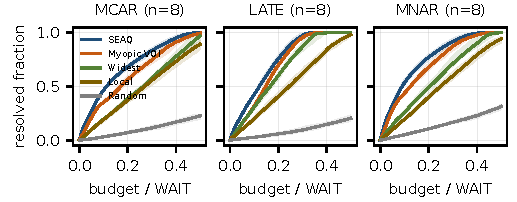
\includegraphics[width=\columnwidth]{g1_resolution.pdf}
\caption{Resolved fraction of initially undetermined decisions versus acquisition budget on the real panel (mean over
$n$ episodes, band = min--max over episodes), plotted from the stored per-episode curves.}\label{fig:g1}\end{figure} \seaq{} has the highest AUC in every cell, and every paired CI excludes
zero. Three observations stand out.
(1)~\emph{Myopic VOI is the strongest baseline but is beaten consistently.} Its gap to \seaq{} is
\daucReallatevoiOne--\daucRealmcarvoiOne{} AUC on real data, and every paired CI excludes zero. Adding the VOI
term to \seaq{} \emph{hurts} (SEAQ+VOI). This is the empirical face of Lemma~\ref{lem:nopartial}: one-probe resolution
probabilities are zero for most inputs and push probes toward decisions that happen to be nearly resolved.
(2)~\emph{Normalisation matters more than sharing.} Widest-first, the TRAPP-style rule, trails by
\daucReallatewidest--\daucRealmcarwidest, and Local per-query probing trails by more. In contrast, removing sharing (SEAQ-noshare) costs only
\daucRealmcarseaqmax--\daucReallateseaqmax{} AUC. The gain from sharing is real (CIs exclude zero) but \emph{small} on this
workload, in which each input feeds at most 8 decisions. Section~\ref{sec:fanout} tests whether it grows with fan-out; it does not.
(3)~\emph{The ordering is the same on real and synthetic data}, under adversarial MNAR missingness, and with heterogeneous probe costs (Real-het columns), where \seaq{} again has the highest AUC in all three scenarios.
A handful of acquisition runs certified a decision wrongly (at most 3 per scenario across all policies). Each was
traced to a violated domain bound, so the soundness assumption, not the policy, failed.

\subsection{End-to-end stream replay}
\label{sec:stream}
We replay the real panel as a stream of \stEvents{} evidence events: for each item, an on-time exact report (40\%),
a late exact report (30\%, geometric delay), or an approximate report followed later by the exact value (30\%).
In addition, \stRestated{} items (0.2\%) are later \emph{restated} by $\times0.6$ or $\times1.5$ to model trade busts and
corrections. Ground truth is the final restated value. Eight decision families (2 windows $\times$ 2 thresholds
$\times$ stock/industry) are evaluated every day. That is \stcertTotal{} decisions.
\begin{table}[t]
\centering
\caption{Stream replay on the real panel (one replay, seed 7). Wrong = wrong when first emitted. Delay = days after
window close. Reversals = later changes of an emitted decision; Flagged = reversals attributable to a detected
contradiction.}
\label{tab:stream}
\scriptsize
\setlength{\tabcolsep}{2pt}
\begin{tabular}{lccc}
\toprule
 & POINT (impute) & WAIT (complete) & CERT (ours)\\
\midrule
Wrong at emission (\%) & \stpointWrongPct & \stwaitWrongPct & \stcertWrongPct\\
Wrong at emission (count) & \stpointWrong & \stwaitWrong & \stcertWrong\\
Mean delay (days) & \stpointDelay & \stwaitDelay & \stcertDelay\\
Emitted on time (\%) & \stpointOnTime & \stwaitOnTime & \stcertOnTime\\
Reversals & \stpointRev & \stwaitRev & \stcertRev\\
\quad of which flagged & \stpointFlag & \stwaitFlag & \stcertFlag\\
\midrule
Throughput (k ev/s) & \tputpoint & -- & \tputcert{} (recomp.\ \tputrecomp)\\
\bottomrule
\end{tabular}
\end{table}
Table~\ref{tab:stream} shows the trade-off that motivates the operator. POINT is always on time but wrong
\stpointWrongPct\% of the time, and it reverses \stpointRev{} decisions without explanation. WAIT is almost never wrong
but arrives \stwaitDelay{} days late on average. CERT emits most decisions on time (\stcertOnTime\%), with a
mean delay of \stcertDelay{} days. Its residual errors (\stcertWrong) are caused by restatements and violated bounds, i.e.\ by
\emph{unsound} evidence, which no evidence-based method can anticipate. Every CERT reversal is attributable to a
detected contradiction. Incremental maintenance of two bounds runs at \tputcert{}k events/s versus \tputpoint{}k
for a point engine (about 1.9$\times$ overhead) and \tputrecomp{}k for recompute-on-change. All numbers are
single-threaded Python. Absolute throughput is not the claim; the ratios are.

\subsection{Where do certified errors come from?}
\begin{table}[t]\centering\caption{Where certified errors come from (stream replay, seed 7). Bound = declared domain bound for unreported items (multiple of calibration max). Violating items = items whose true value exceeds the bound.}\label{tab:sound}
\scriptsize\setlength{\tabcolsep}{2pt}\begin{tabular}{lrrrrr}\toprule
Bound, restat. & Viol. & CERT err & on-time \% & delay (d) & WAIT err\\
\midrule
$3\times$, restat. (main) & 1364 & 397 & 62.9 & 0.84 & 344\\
$3\times$, no restat. & 1363 & 36 & 62.8 & 0.84 & 0\\
$10\times$, restat. & 183 & 364 & 57.8 & 1.00 & 344\\
$10\times$, no restat. & 183 & 7 & 57.7 & 1.00 & 0\\
$1000\times$, no restat. & 0 & 0 & 53.4 & 1.17 & 0\\
\bottomrule\end{tabular}\end{table}

Proposition~\ref{prop:sound} says certified errors \emph{require} unsound evidence. Table~\ref{tab:sound} tests this by
removing the two sources of unsoundness one at a time. Without restatements, the only errors left are those from
items whose true value exceeds the declared $3\times$ bound. Raising the bound to $10\times$ removes most violations
and the corresponding errors, but it costs on-time coverage, because wider bounds certify less. With restatements
on, WAIT is wrong about as often as CERT: a restated input invalidates any decision taken before the restatement,
however complete the data looked. Contradiction detection (Proposition~\ref{prop:sound}(c)) turns each such case into
a flagged retraction, but it cannot prevent the initial error. When both sources of unsoundness are removed ($1000\times$ bounds, no violating items, no restatements), CERT made
\emph{zero} wrong certifications, but on-time emission fell from 62.9\% to 53.4\%. Every observed error is therefore
attributable to an explicit assumption violation. Retraction repairs an error \emph{after} it happened and does not
prevent it. The guarantee is therefore exactly as strong as the declared bounds, and choosing the bound trades coverage
against safety.

\subsection{Controlled fan-out: when does sharing matter?}
\label{sec:fanout}
\begin{table*}[t]\centering\caption{Controlled fan-out benchmark: 1024 decisions of 32 items each, every item feeds exactly $f$ decisions (5 instances per $f$). Mean AUC; last columns: AUC gain of \seaq{} over SEAQ-noshare and over myopic VOI with min--max over instances, \seaq{} C90, and \seaq{} runtime.}\label{tab:fanout}
\scriptsize\setlength{\tabcolsep}{2pt}\begin{tabular}{rrcccccccccr}\toprule
$f$ & items & Rand & Widest & Deg & VOI & noshare & \seaq & $\Delta$noshare & $\Delta$VOI & C90 & s\\
\midrule
1 & 32768 & 0.011 & 0.013 & 0.012 & 0.316 & 0.316 & 0.316 & +0.000 [+0.000,+0.000] & +0.000 [-0.001,+0.001] & 0.838 & 2.5\\
2 & 16384 & 0.011 & 0.015 & 0.013 & 0.172 & 0.198 & 0.202 & +0.005 [+0.002,+0.007] & +0.031 [+0.029,+0.032] & 0.911 & 1.5\\
4 & 8192 & 0.013 & 0.015 & 0.015 & 0.102 & 0.121 & 0.127 & +0.006 [+0.003,+0.009] & +0.025 [+0.023,+0.026] & 0.931 & 0.5\\
8 & 4096 & 0.010 & 0.011 & 0.010 & 0.060 & 0.072 & 0.075 & +0.003 [-0.000,+0.006] & +0.015 [+0.013,+0.016] & 0.956 & 0.3\\
16 & 2048 & 0.010 & 0.010 & 0.009 & 0.034 & 0.042 & 0.043 & +0.001 [-0.002,+0.004] & +0.009 [+0.006,+0.012] & 0.969 & 0.1\\
32 & 1024 & 0.010 & 0.009 & 0.008 & 0.028 & 0.026 & 0.026 & -0.000 [-0.004,+0.001] & -0.002 [-0.011,+0.003] & 0.978 & 0.1\\
\bottomrule\end{tabular}\end{table*}

The real workload gives each input a fan-out of at most 8. To test whether sharing matters more at higher fan-out,
we built a controlled benchmark that varies only the sharing structure. It has 1024 decisions of 32 items each, and every
item feeds exactly $f$ decisions in a random regular design. Missingness is 50\%, missing items carry the bound
$[0,4\mu]$, item values are Gamma-distributed with per-item mean $\mu$, and thresholds are $\theta_d=|S_d|\,\mu\cdot U(0.9,1.1)$, i.e.\ within
$\pm10\%$ of the decision's expected sum. This is the formula implemented in \texttt{run\_fanout.py}, and all 1024 decisions start
undetermined. Decision count,
decision size, missingness and threshold rule are fixed. The item pool necessarily shrinks as $D\cdot s/f$.
Table~\ref{tab:fanout} \emph{refutes} the hypothesis that the benefit of sharing grows with fan-out. The gain of
\seaq{} over SEAQ-noshare peaks at $f=2$--$4$ (at most $+0.006$) and is indistinguishable from zero for $f\ge 16$. The gain
over myopic VOI is largest at $f=2$ ($+0.031$) and shrinks to zero at $f=32$. At $f=1$ (no sharing) \seaq, VOI and
noshare coincide. More importantly, every policy degrades as $f$ grows. Each decision then depends on inputs that
are also uncertain for many other decisions, and with thresholds near the mean, almost all of a decision's
uncertain inputs must be fetched (C90 approaches 1, as Lemma~\ref{lem:nopartial} predicts for adversarial cases).
In that regime, simply fetching everything (WAIT) is as good as any policy. \seaq's measured advantage therefore
comes mainly from \emph{width normalisation} (versus Widest and Degree) and from avoiding myopic VOI's zero
scores at low-to-moderate fan-out. It does not come from exploiting sharing.

\subsection{Exact guaranteed-resolution planning}
\label{sec:wc}
\begin{table}[t]\centering\caption{Guaranteed-resolution planning on the real panel (stock-level windows, 40-day backlog, 5 days per scenario). Row 1: optimum number of decisions guaranteed resolved (exact DP, Thm.~\ref{thm:dp}), mean over days. Other rows: fraction of the optimum achieved by each non-adaptive plan at the same budget (budget = fraction of total uncertain-item cost).}\label{tab:wc}
\scriptsize\setlength{\tabcolsep}{2.2pt}\begin{tabular}{llccccc}\toprule
Scen. & Plan & 2\% & 5\% & 10\% & 20\% & 40\%\\
\midrule
LATE & \textbf{Exact DP (count)} & 527 & 1153 & 2040 & 3527 & 5755\\
 & Greedy cheapest-completion & 0.52 & 0.67 & 0.66 & 0.74 & 0.83\\
 & Completion score & 0.41 & 0.44 & 0.51 & 0.61 & 0.75\\
 & \seaq{} order & 0.11 & 0.08 & 0.08 & 0.11 & 0.22\\
 & Widest order & 0.06 & 0.06 & 0.08 & 0.13 & 0.20\\
 & Random & 0.00 & 0.01 & 0.01 & 0.02 & 0.05\\
 & \multicolumn{6}{l}{decisions: 7475; exact DP time: 0.66 s}\\
\midrule
MCAR & \textbf{Exact DP (count)} & 1088 & 2584 & 4946 & 9369 & 17464\\
 & Greedy cheapest-completion & 0.54 & 0.58 & 0.71 & 0.86 & 0.90\\
 & Completion score & 0.27 & 0.23 & 0.22 & 0.23 & 0.44\\
 & \seaq{} order & 0.04 & 0.03 & 0.03 & 0.04 & 0.08\\
 & Widest order & 0.06 & 0.06 & 0.06 & 0.07 & 0.11\\
 & Random & 0.00 & 0.00 & 0.01 & 0.01 & 0.05\\
 & \multicolumn{6}{l}{decisions: 32837; exact DP time: 1.31 s}\\
\bottomrule\end{tabular}\end{table}

Fig.~\ref{fig:g2} plots the guaranteed counts.
\begin{figure}[t]\centering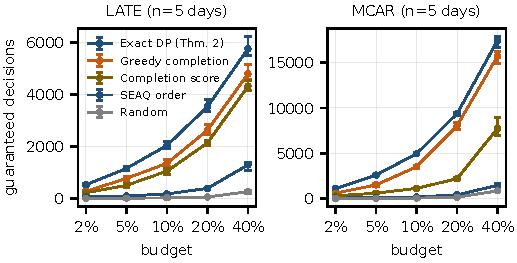
\includegraphics[width=\columnwidth]{g2_exact.pdf}
\caption{Decisions guaranteed resolved versus budget: exact optimum (Thm.~\ref{thm:dp}) and non-adaptive heuristic plans
(mean over 5 days, bars = min--max). The exact curve is an optimum, not an estimate; the others are measured plans.}\label{fig:g2}\end{figure}
We build a 40-day backlog of stock-level windows on the real panel ($W\in\{5,20\}$, two thresholds, windows ending on
each of the last 40 days; about 7.5k (LATE) and 33k (MCAR) undetermined decisions). We compare the exact plan of
Theorem~\ref{thm:dp} with non-adaptive plans of the same cost. Table~\ref{tab:wc} gives the answer. The best heuristic,
a classic cheapest-completion greedy, reaches only 52--54\% of the optimum at a 2\% budget and 83--90\% at 40\%. Plans
ordered by \seaq{} or width reach at most 22\%, because those scores spread probes across decisions instead of
completing them. The exact optimiser solves the whole panel in about 0.7--1.3\,s in Python. This is the
capability the paper adds beyond bound propagation: an acquisition plan with a \emph{guaranteed} and \emph{provably
maximal} number of settled alerts. The two objectives call for different tools. \seaq{} is the right policy for
\emph{expected} resolution (Table~\ref{tab:acq}); the exact plan is the right one for \emph{commitments}.

\textbf{With roll-ups.} Table~\ref{tab:rollup} adds the industry roll-up decisions and solves the full problem
exactly with the ILP. HiGHS proved optimality in 15--30\,s on every instance. Two findings stand out. First, roll-up
decisions are rarely worth guaranteeing: each needs every member's uncertain slots, so the optimum settles only a few
dozen of the 380--610 roll-ups. Second, the plan of the window DP, which ignores roll-ups, reaches at least 99\% of the
full optimum at about 1\,s. The greedy completion plan reaches 66--76\%, and \seaq{}/width orders reach at most 14\%. On
this workload the tractable class therefore captures almost all of the achievable guarantee, and an exact ILP
certifies the remaining gap. We expect the gap to grow when roll-ups dominate (small groups, few uncertain members),
which we did not test.
\begin{table}[t]\centering\caption{Guaranteed-resolution planning with industry roll-ups (real panel, LATE, 40-day backlog, 3 days). Entries: stock + industry decisions guaranteed (mean over days), ratio to the exact optimum in parentheses. The ILP proved optimality on all 6 solves in 15--30\,s; the window DP (Thm.~\ref{thm:dp}) takes 1.1\,s, the value-indexed DP with real-valued costs 0.75\,s. Mean decisions: 7294 stock + 503 industry.}\label{tab:rollup}
\scriptsize\setlength{\tabcolsep}{3pt}\begin{tabular}{lcc}\toprule
Plan & 5\% budget & 20\% budget\\
\midrule
Exact ILP (HiGHS) & 1133+13 (1.000) & 3438+41 (1.000)\\
Window DP, stock only & 1141+3 (0.998) & 3454+3 (0.994)\\
Greedy completion & 759+3 (0.664) & 2556+6 (0.737)\\
\seaq{} order & 110+3 (0.098) & 411+4 (0.120)\\
Widest order & 78+1 (0.070) & 439+5 (0.128)\\
\bottomrule\end{tabular}\end{table}


\textbf{Negative result: completion scores do not help expected resolution.} Motivated by GR, we also tested an
adaptive completion-oriented score ($\sum_d 1/r_d$, where $r_d$ is the number of uncertain items left in $d$) and an
equal-weight hybrid with \seaq{}. These were added after the v1 freeze and evaluated on the same real episodes, so the
test is exploratory. On real data the completion score loses to \seaq{} by 0.156--0.223 AUC, and the hybrid by
0.002--0.005 (all CIs exclude zero). On the fan-out benchmark both tie with \seaq{}, and neither repairs the
high-fan-out failure. \seaq{} stays the expected-resolution policy.

\subsection{System prototype: CQP on DuckDB}
\label{sec:cqp}
To test the operator as database functionality and not only as Python arrays, we built CQP, a certified
decision-query processor whose entire state lives in SQL tables in DuckDB~1.1.3. These tables hold evidence intervals,
registered queries and per-entity thresholds, materialised decisions $(L,U,\text{state},\text{emitted})$, and decision,
retraction, contradiction and acquisition logs. Ingestion is one SQL pipeline per batch. It first detects
contradictions by joining the batch against stored evidence and testing interval disjointness. It then builds a
per-slot delta $(\Delta\ell,\Delta h)$ and applies it with one \texttt{UPDATE \dots FROM} to every stock and roll-up window
containing the slot. Finally it computes state transitions, emissions and retractions; each retraction records whether a
contradiction in the same batch touched the window. \seaq{} is a single SQL aggregation over (uncertain item
$\times$ undetermined window), and the exact planner of Theorem~\ref{thm:dp} reads its slots and ranges from SQL.
\texttt{explain()} reports, for an insufficient decision, its gaps to both outcomes and its widest contributing items.

\textbf{Tests} (\texttt{cqp/test\_cqp.py}, 9/9 pass in a fresh Python~3.12 virtual environment with pinned
dependencies). The tests check that (1) incremental state equals full SQL window-function recomputation after random
batches; (2) states match the reference semantics; (3) no certified decision is wrong under sound bounds; (4) a
disjoint restatement is detected and every resulting retraction is flagged as contradiction-caused; (5) sound
narrowing never causes a retraction (Prop.~\ref{prop:sound}(b)); (6) the SQL \seaq{} scores equal the NumPy
reference on every item; (7) every decision counted by the exact plan is resolved under 50 random outcomes of the
planned probes; (8) the plan is optimal against brute force on a small instance; and (9) the three engine modes below produce
identical states and logs. \textbf{Demo}
(\texttt{cqp/demo.py}) is deterministic and needs no external data. It covers two sources and three stocks in one
industry, with missing and approximate evidence, insufficient alerts, \seaq{} acquisition, a guaranteed-resolution
plan, and a late restatement (a trade bust). The restatement produced 5 retractions, all flagged; the demo then
checks the results: no certified decision is wrong against the final truth, and the incremental and full states
agree to $2\times10^{-13}$.

\textbf{Real-panel benchmark with equivalent functionality} (\texttt{cqp/bench.py}, \texttt{cqp/bench\_repeat.sh},
Table~\ref{tab:cqp}). CQP has three engine modes with \emph{identical observable semantics}: the same contradiction
check, states, emissions, retractions and logs. In \emph{full} mode the bounds are recomputed from scratch by SQL window
functions inside the same transaction. In \emph{inc\_scan} mode the bounds are maintained by deltas and the transition
step scans all decisions; in \emph{inc} mode the transition step is restricted to the decisions touched by the delta.
Test (9) checks the equivalence on randomized batches with contradictions. Each mode ran 5 times (Fig.~\ref{fig:g3}), every run in a fresh
process with a fresh database, with the mode order rotated across runs. Batches, engine, data layout, query set and
machine were identical. We treat the run, not the batch, as the unit of replication. All 15 runs produced identical state
digests and log counts. Delta maintenance is 2.30--2.37$\times$ faster than equivalent full recomputation in total time
(2.30--2.44$\times$ at the median batch), and the range across runs is narrow. The affected-only and scan transition steps are
indistinguishable (p50 398 vs.\ 404\,ms). Restricting transitions saves nothing here because each changed slot feeds up
to 20 windows per query, so a large share of decisions is touched per batch. Hence the $O(\deg)$ update bound does not
by itself yield an end-to-end gain beyond the delta-versus-recompute difference. A first, single, 120-day run under
\texttt{DOUBLE} arithmetic gave p50 540/620/1046\,ms (scan/affected/full) and a p95 for affected-only (1186\,ms) above
full recomputation (1119\,ms). We report it as superseded, single-run evidence (\texttt{results/cqp\_bench\_120d\_*.json}).
The gains over plain SQL are therefore the semantics (emission, retraction attribution, abstention reasons) and a
consistent $\sim$2.3$\times$ latency advantage at this scale; we did not test other scales or engines.
\begin{table*}[t]\centering\caption{Repeated equivalent-functionality benchmark on DuckDB~1.1.3, exact integer arithmetic (398 stocks, 60 days, 8 queries, 81,092 decisions, 63 daily batches). 5 runs per mode; each run is a fresh process and a fresh database, and the mode order is rotated across runs. Entries: median over runs [min--max over runs] of the per-run statistic. All 15 runs produced identical state digests and log counts. Speedup of total time, full over incremental-scan: 2.32 [2.30--2.37].}\label{tab:cqp}
\scriptsize\setlength{\tabcolsep}{1.5pt}\begin{tabular}{lcccc}\toprule
Mode & p50 (ms) & p95 (ms) & p99 (ms) & total (s)\\
\midrule
Incremental, transition scan & 404 [396--406] & 675 [656--684] & 706 [688--707] & 25.6 [25.4--25.8]\\
Incremental, affected-only & 398 [391--409] & 659 [646--683] & 701 [655--703] & 25.2 [25.0--25.5]\\
Full SQL recompute, same semantics & 950 [931--968] & 1051 [1040--1059] & 1079 [1069--1093] & 59.4 [59.0--60.2]\\
\bottomrule\end{tabular}\end{table*}

\begin{figure}[t]\centering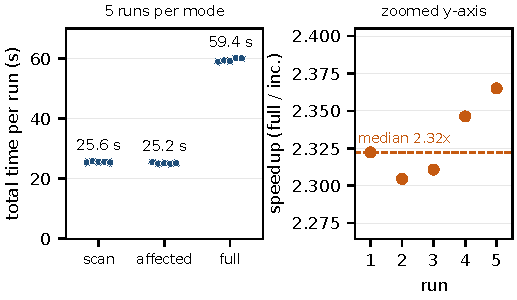
\includegraphics[width=\columnwidth]{g3_bench.pdf}
\caption{Repeated DuckDB benchmark (60 days, 8 queries, 5 runs per mode, each a fresh process and database). Left (modes: incremental scan, incremental affected-only, full recomputation):
total time of every run (dots) and observed min--max range (bar), axis from 0, label = median. Right: paired speedup of
full recomputation over incremental (scan) per run; the y-axis is zoomed and does not start at 0. Data:
\texttt{results/cqp\_bench\_60d\_*\_rep*.json}.}\label{fig:g3}\end{figure}

\textbf{Numerical soundness.} The first version stored bounds as \texttt{DOUBLE}. Incremental and full bounds then
differed by up to $10^{-4}$, because approximate readings produce non-integer bounds, and floating-point summation is
order-dependent. Near a threshold such a drift could flip a certified state, so CQP now certifies in \emph{exact integer
arithmetic}. Traded volumes are integers. An evidence interval $[\ell,h]$ is therefore replaced by its integer hull
$[\lceil\ell\rceil,\lfloor h\rfloor]$, which is sound because the true value is an integer in $[\ell,h]$ and is never
looser. A threshold $\theta$ is replaced by $\lfloor\theta\rfloor$, which is exact for integer sums: $L>\theta \iff
L>\lfloor\theta\rfloor$ and $U\le\theta\iff U\le\lfloor\theta\rfloor$. All bounds are \texttt{BIGINT}, so incremental and
full recomputation now agree \emph{exactly}, and certification involves no rounding. Evidence whose integer hull is
empty (for example an ``exact'' non-integer volume) is rejected as a violation of the domain assumption. A threshold is
taken at its exact binary value: $2\cdot10^{12}+0.999999$ is the double $2\cdot10^{12}+1$, and a test documents this.
A separate suite (\texttt{cqp/test\_numeric.py}, 7 tests) checks equality at the lower and upper bounds, one integer
step on either side, fractional thresholds with outward rounding, values near zero, magnitudes of $10^{12}$, and 30
batches of updates with contradictions in all three engine modes. It checks every state against an independent
Python-integer reference and requires exact agreement. Together with the 9 engine tests, 16/16 pass in a fresh
environment. Non-integer domains would need outward-rounded interval arithmetic, which we do not implement.

\textbf{Theory-to-system contract.} Prop.~\ref{prop:sound} corresponds to \texttt{engine.ingest} and tests (3)--(5).
Lemma~\ref{lem:nopartial} and Thm.~\ref{thm:dp} correspond to \texttt{acquire\_sql.gr\_plan} and tests (7)--(8), and
Thm.~\ref{thm:hard} explains why roll-ups fall back to the ILP (\texttt{run\_rollup.py}). The \seaq{} score is
\texttt{acquire\_sql.SEAQ\_SQL}, checked by test (6).

\subsection{Limits and threats to validity}
\label{sec:limits}
\emph{Soundness is conditional:} certification is only as good as the declared bounds. Domain bounds at
$3\times$ the calibration maximum were violated for some items, and then decisions can be certified wrongly
(Table~\ref{tab:zero}, Section~\ref{sec:stream}). Contradiction detection catches a violation only once
disjoint evidence arrives. \emph{Wide bounds are expensive:} with uninformative domain bounds only about 20\% of
decisions certify without probing. Tighter, validated bounds (e.g.\ from circuit limits or historical quantiles)
would help but would weaken the guarantee. \emph{Prototype scope:} CQP is an external SQL-backed operator on DuckDB, not
an engine-internal operator. Its incremental path is about $2.3\times$ faster than equivalent full recomputation on one panel size and
one engine; restricting transitions to affected decisions gives no further gain (Section~\ref{sec:cqp}). \emph{Scope of operators:} we evaluate SUM thresholds only. Joins with
uncertain keys and non-monotone aggregates (AVG with uncertain counts) are not covered. \emph{Sharing:} the
measured benefit of sharing is small on real data and does not grow with fan-out in the controlled benchmark
(Table~\ref{tab:fanout}). \emph{Costs:} unit costs in the main table; probe costs in practice
depend on the source. \emph{Statistics:} 8--12 episodes per cell. The CIs are over episodes for a single panel
and seed family, and the stream replay is a single seed. \emph{No worst-case guarantee} for \seaq{}
(Theorem~\ref{thm:hard} suggests none is cheap). \emph{Generality:} the formulation is domain-agnostic (sensor
alerts, SLA checks, fraud rules), but we evaluated only volume alerts on Indian equities plus synthetic data.

\section{What Is and Is Not New}
\label{sec:novelty}
\emph{Known, reused:} the certified semantics (certain answers~\cite{imielinski1984,libkin2016}; attribute bounds as in
AU-DBs~\cite{feng2021audb}); delta-based maintenance~\cite{gupta1993}; the gap-decomposition and min-plus convolution
techniques inside the planner; the 0-1 ILP formulation; and Densest-$k$-Subgraph hardness~\cite{feige2001dks}.
\emph{New formulation:} \emph{guaranteed-resolution} (GR) acquisition for many threshold decisions sharing interval
evidence. It differs from TRAPP~\cite{olston2000trapp} (one aggregate, a width target), from probing~\cite{cheng2003} and
QOCO~\cite{bergman2015qoco} (single queries or answer sets), and from stochastic Boolean function
evaluation~\cite{deshpande2014sbfe} (one function, expected cost). Budgeted maximum coverage does not apply directly,
because a decision is ``covered'' only by \emph{all} of its uncertain inputs (Lemma~\ref{lem:nopartial}), which makes
the objective a conjunctive, DkS-like one. \emph{New results:} Lemma~\ref{lem:nopartial} and its consequences; NP-hardness of
adaptive and non-adaptive GR (Thm.~\ref{thm:hard}); strong polynomiality of GR for window workloads (Thm.~\ref{thm:dp}),
together with the line drawn by roll-ups; and the empirical finding that heuristics, including our own \seaq{}, reach
only 52--54\% (best case) of the GR optimum at low budgets. \emph{New system:} CQP, with contradiction-attributed
retractions, SQL-native \seaq{} and the planner, and three engine modes proven observably equivalent by test.
\emph{Not new:} \seaq's score is a normalised-width heuristic. Its value is empirical (Table~\ref{tab:acq}), and the
fan-out benchmark shows where that value comes from.

\section{Related Work}
\label{sec:related}
\emph{Incomplete and uncertain data.} Certain answers and Codd-table semantics~\cite{imielinski1984}, SQL's
three-valued logic versus certainty~\cite{libkin2016}, consistent query answering~\cite{arenas1999}, probabilistic
databases~\cite{dalvi2004}, compact world-set representations~\cite{antova2007}, and UA-/AU-DBs with attribute-level
bounds~\cite{feng2019uadb,feng2021audb} define \emph{what} is certain. Our semantics is a special case of these. Our
contribution concerns maintaining it for windowed threshold decisions and \emph{acquiring} evidence to resolve them.
\emph{Precision-aware refresh and probing.} TRAPP~\cite{olston2000trapp} and adaptive filters~\cite{olston2003filters}
choose which cached values to refresh so that a single (continuous) aggregate meets a precision bound. Cheng et
al.~\cite{cheng2003} evaluate and probe imprecise values, and QOCO~\cite{bergman2015qoco} asks oracles to clean answers of
a given query. We differ in the objective (number of resolved \emph{threshold decisions} rather than the width of one answer) and in
sharing an input across many decisions. Widest and Local are our implementations of their single-query
principle, and we show they are dominated in this setting.
\emph{Stream processing.} CQL~\cite{arasu2006cql} defines windowed continuous queries. The Dataflow
model~\cite{akidau2015dataflow} handles lateness with watermarks and retractions, which corresponds to our WAIT and POINT
engines. Distributed threshold monitoring with safe zones~\cite{sharfman2006} minimises communication for one global
function under exact local values. Incremental view maintenance~\cite{gupta1993} underlies our delta updates.
\emph{Provenance and cleaning.} Why-provenance~\cite{buneman2001} and semiring provenance~\cite{green2007} explain
answers. ActiveClean~\cite{krishnan2016activeclean} and stale-view cleaning~\cite{krishnan2015stale} prioritise cleaning
for model or view accuracy, and online aggregation~\cite{hellerstein1997online} trades accuracy for time.
\emph{Theory.} Stochastic Boolean function evaluation~\cite{deshpande2014sbfe} studies adaptive evaluation of one
threshold function, and Densest-$k$-Subgraph~\cite{feige2001dks} gives our hardness result.

\section{Reproducibility}
\label{sec:repro}
\emph{Prototype:} \texttt{pip install -r requirements.txt} (pinned versions: Python~3.12, DuckDB~1.1.3, NumPy~2.2.6,
SciPy~1.15.3), then \texttt{python -m pytest cqp/test\_cqp.py}, \texttt{python cqp/demo.py} and
\texttt{bash cqp/bench\_repeat.sh} (5 runs $\times$ 3 modes, 60 days; produces Table~\ref{tab:cqp} and Fig.~\ref{fig:g3} via
\texttt{cqp/make\_repeat\_table.py} and \texttt{src/make\_graphs.py}; \texttt{python cqp/bench.py 120 inc} reproduces the superseded single run), \texttt{python -m pytest cqp/test\_numeric.py}. We ran these in a freshly created virtual environment and they completed as reported. A
Dockerfile is included but was \emph{not} built or tested: the Docker CLI is installed but the daemon was not
running (\texttt{docker info}: cannot connect), so we claim no container reproducibility. DuckDB~2.0.0 under Python~3.14 raised an internal assertion (``dict-surviving cache'') in
the delta-update query on the full panel but not on small inputs. We did not isolate a minimal reproduction, and we pin
DuckDB~1.1.3, the only version tested end to end.
\emph{Algorithms and tables:}
The artifact contains \texttt{src/} (operator \texttt{cert.py}, policies \texttt{acquire.py}, workloads
\texttt{workload.py}, experiments \texttt{run\_acq.py}, \texttt{run\_stream.py}, number generation
\texttt{make\_numbers.py}) and \texttt{DEV\_LOG.md} with the freeze and SHA-256 hashes. All numbers in this paper are
macros generated from \texttt{results/*.json}. Commands: \texttt{python run\_acq.py real 8 --tag main};
\texttt{python run\_acq.py synth 12 --seed 3 --tag main}; \texttt{python run\_stream.py 7};
\texttt{python run\_fanout.py}; \texttt{python wcdp.py} (DP vs.\ brute force);
\texttt{python run\_wc.py}; \texttt{python make\_wc.py}; \texttt{python wcdp\_sp.py};
\texttt{python run\_rollup.py}; \texttt{python make\_rollup.py}; \texttt{python verify\_theory.py};
\texttt{CAP\_MULT=10 python run\_stream.py 7 0.3 0.3 0.0} (and the other three soundness settings);
\texttt{python make\_numbers.py}; \texttt{python make\_table.py}; \texttt{python make\_extra.py}. The exchange files are public, but we do not redistribute them; the
original download scripts and checksums are included. Hardware: a 12-thread Windows~11 laptop with 7.7\,GB RAM, Python
3.14, NumPy 2.5, SciPy 1.18. Every run in the paper completes in minutes.

\section{Conclusion}
Treating threshold queries as \emph{decisions} over bounded evidence separates what a monitoring engine can certify
from what it is guessing. The certified state is cheap to maintain incrementally. Resolving the rest is
combinatorially hard in the worst case, but a shared, normalised progress score resolves decisions with
substantially less acquisition than single-query refresh rules or myopic VOI. For window workloads, guaranteed-resolution plans can be
optimised exactly and fast, and heuristics fall far short of the optimum. Two further findings matter for practice. Certified errors arise only from unsound evidence (violated bounds and
restatements), and bound width trades coverage against safety. Shared acquisition helps at low-to-moderate fan-out
but not at high fan-out, where fetching everything is as good. The open problems are validated tight bounds,
operators beyond SUM, and an acquisition objective that actually benefits from sharing.

\section*{Acknowledgment and AI-Generated Content Disclosure}
An AI assistant (Anthropic Claude) assisted with code, experiments and drafting under the authors' direction; the
authors take full responsibility for the content.

\bibliographystyle{IEEEtran}
\bibliography{refs}
\end{document}
